\documentclass[a4paper, 11pt, oneside]{article}

\usepackage[utf8]{inputenc}
\usepackage[T1]{fontenc}
\usepackage[french]{babel}
\usepackage{array}
\usepackage{shortvrb}
\usepackage{listings}
\usepackage[fleqn]{amsmath}
\usepackage{amsfonts}
\usepackage{fullpage}
\usepackage{enumerate}
\usepackage{graphicx}             % import, scale, and rotate graphics
\usepackage{subfigure}            % group figures
\usepackage{alltt}
\usepackage{url}
\usepackage{indentfirst}
\usepackage{eurosym}
\usepackage{listings}
\usepackage{color}
\usepackage[table,xcdraw,dvipsnames]{xcolor}

% Change le nom par défaut des listing
\renewcommand{\lstlistingname}{Extrait de Code}

% Change la police des titres pour convenir à votre seul lecteur
\usepackage{sectsty}
\allsectionsfont{\sffamily\mdseries\upshape} 
% Idem pour la table des matière.
\usepackage[nottoc,notlof,notlot]{tocbibind} 
\usepackage[titles,subfigure]{tocloft} 
\renewcommand{\cftsecfont}{\rmfamily\mdseries\upshape}
\renewcommand{\cftsecpagefont}{\rmfamily\mdseries\upshape} 

\definecolor{mygray}{rgb}{0.5,0.5,0.5}
\newcommand{\coms}[1]{\textcolor{MidnightBlue}{#1}}

\lstset{
    language=C, % Utilisation du langage C
    commentstyle={\color{MidnightBlue}}, % Couleur des commentaires
    frame=single, % Entoure le code d'un joli cadre
    rulecolor=\color{black}, % Couleur de la ligne qui forme le cadre
    stringstyle=\color{RawSienna}, % Couleur des chaines de caractères
    numbers=left, % Ajoute une numérotation des lignes à gauche
    numbersep=5pt, % Distance entre les numérots de lignes et le code
    numberstyle=\tiny\color{mygray}, % Couleur des numéros de lignes
    basicstyle=\tt\footnotesize, 
    tabsize=3, % Largeur des tabulations par défaut
    keywordstyle=\tt\bf\footnotesize\color{Sepia}, % Style des mots-clés
    extendedchars=true, 
    captionpos=b, % sets the caption-position to bottom
    texcl=true, % Commentaires sur une ligne interprétés en Latex
    showstringspaces=false, % Ne montre pas les espace dans les chaines de caractères
    escapeinside={(>}{<)}, % Permet de mettre du latex entre des <( et )>.
    inputencoding=utf8,
    literate=
  {á}{{\'a}}1 {é}{{\'e}}1 {í}{{\'i}}1 {ó}{{\'o}}1 {ú}{{\'u}}1
  {Á}{{\'A}}1 {É}{{\'E}}1 {Í}{{\'I}}1 {Ó}{{\'O}}1 {Ú}{{\'U}}1
  {à}{{\`a}}1 {è}{{\`e}}1 {ì}{{\`i}}1 {ò}{{\`o}}1 {ù}{{\`u}}1
  {À}{{\`A}}1 {È}{{\`E}}1 {Ì}{{\`I}}1 {Ò}{{\`O}}1 {Ù}{{\`U}}1
  {ä}{{\"a}}1 {ë}{{\"e}}1 {ï}{{\"i}}1 {ö}{{\"o}}1 {ü}{{\"u}}1
  {Ä}{{\"A}}1 {Ë}{{\"E}}1 {Ï}{{\"I}}1 {Ö}{{\"O}}1 {Ü}{{\"U}}1
  {â}{{\^a}}1 {ê}{{\^e}}1 {î}{{\^i}}1 {ô}{{\^o}}1 {û}{{\^u}}1
  {Â}{{\^A}}1 {Ê}{{\^E}}1 {Î}{{\^I}}1 {Ô}{{\^O}}1 {Û}{{\^U}}1
  {œ}{{\oe}}1 {Œ}{{\OE}}1 {æ}{{\ae}}1 {Æ}{{\AE}}1 {ß}{{\ss}}1
  {ű}{{\H{u}}}1 {Ű}{{\H{U}}}1 {ő}{{\H{o}}}1 {Ő}{{\H{O}}}1
  {ç}{{\c c}}1 {Ç}{{\c C}}1 {ø}{{\o}}1 {å}{{\r a}}1 {Å}{{\r A}}1
  {€}{{\euro}}1 {£}{{\pounds}}1 {«}{{\guillemotleft}}1
  {»}{{\guillemotright}}1 {ñ}{{\~n}}1 {Ñ}{{\~N}}1 {¿}{{?`}}1
}
\newcommand{\tablemat}{~}

%%%%%%%%%%%%%%%%% TITRE %%%%%%%%%%%%%%%%
\newcommand{\intitule}{Projet 1 Rapport}
\newcommand{\GrNbr}{10}
\newcommand{\PrenomUN}{Cyril}
\newcommand{\NomUN}{Russe}
\newcommand{\PrenomDEUX}{Martin}
\newcommand{\NomDEUX}{Randaxhe}
\renewcommand{\tablemat}{\tableofcontents}

%%%%%%%% ZONE PROTÉGÉE : MODIFIEZ UNE DES DIX PROCHAINES %%%%%%%%
%%%%%%%%            LIGNES POUR PERDRE 2 PTS.            %%%%%%%%
\title{INFO0947: \intitule}
\author{Groupe \GrNbr : \PrenomUN~\textsc{\NomUN}, \PrenomDEUX~\textsc{\NomDEUX}}
\date{}
\begin{document}
\maketitle
\newpage
\tablemat
\newpage
%%%%%%%%%%%%%%%%%%%% FIN DE LA ZONE PROTÉGÉE %%%%%%%%%%%%%%%%%%%%

%%%%%%%%%%%%%%%% RAPPORT %%%%%%%%%%%%%%%

\section{Définition du problème}
\subsection{Introduction}
Soit $T$, un tableau à $N$ valeurs entière $(N \geq 0)$. On veut
construire une fonction qui permet d’obtenir, pour $T$, le plus 
grand entier $k (k\in2 [0,\dots,N-1])$ tel que le sous-tableau 
$T[0\dots k-1]$ est à la fois préfixe et suffixe de $T$. 
Si un tel sous-tableau n’existe pas, la fonction doit renvoyer la 
valeur 0. Attention, on fait l’hypothèse que $k\neq N$ sinon 
le problème devient trivial.
\subsection{Input/Output}
\subsubsection{Input}
\begin{itemize}
  \item $T$ : un tableau d'entier de taille $N$
  \item $N$ : la taille du tableau $T$
\end{itemize}

\subsubsection{Output}
\begin{itemize}
  \item $taille\_sous\_tableau$ : la taille du plus grand sous tableau à la fois préfixe et suffixe de $T$
\end{itemize}

\subsection{Objets utilisés}
\begin{itemize}
  \item int *$T$ : un tableau d'entier de taille $N$
  \item unsigned int $N$ : la taille du tableau d'entier
  \item int $est\_pref\_et\_suf$ : une variable booléenne permettant de savoir si le sous tableau 
  analysé est préfixe et suffixe
  \item int $taille\_sous\_tableau$ : la taille du plus grand sous tableau à la fois préfixe et suffixe de $T$
  \item int $i$, $j$ : des compteurs de boucle
\end{itemize}

\section{Formalisation du problème}

\subsection{Description de notation}
  \begin{itemize}
  \item $MemeSSTableau(T,N,i)\equiv \exists j, 0\leq j\leq i, T[j]\neq T[N-1-i+j]\Rightarrow 0$, sinon $1$
  \item $PrefixeSuffixe(T,N)\equiv i+1$ si $\forall i, 0\leq i< N-1, MemeSSTableau(T, N, i)=1$
  \end{itemize}
\newpage
\subsection{Spécifications}

\begin{lstlisting}[caption={Spécification fonction EgaliteSSTab}]
  /**
  *
  * EgaliteSSTab
  *
  * Fonction qui renvoit la taille du plus grand sous tableau 
  * étant préfixe et suffixe
  *
  * @param  T un tableau d'entiers initialisé au préalable
  * @param  N un entier définissant la taille de T
  *
  * @pre : T!=NULL, N>1
  * @post : T=T_0, N=N_0, taille_sous_tableau = PrefixeSuffixe(T, N)
  *
  * @return : taille_sous_tableau
  */
  int EgaliteSSTab(int *T, const unsigned int N);
  (>\label{code:ret}<)
\end{lstlisting}

\subsection{Décomposition en sous-problèmes}
\begin{itemize}
  \item \textbf{Sous-problème 1} : Teste les préfixes/suffixes de T
en allant de 0 à N-1
  \item \textbf{Sous-problème 2} : Teste si chaque élément préfixe
est égal à l'élément correspondant suffixe 
\end{itemize}
$$SP2\subset SP1$$

\subsection{Spécification des sous-problèmes}
\begin{itemize}
  \item \textbf{SP1} : 
  \begin{itemize}
    \item @pre : $$Tinit\wedge T\neq NULL \wedge N>1 \wedge i=0 \wedge taille\_sous\_tableau=0 \wedge est\_pref\_et\_suf=1$$
    \item @post : $$T=T_0\wedge N=N_0\wedge taille\_sous\_tableau=PrefixeSuffixe (T, N)$$
  \end{itemize}
  \item \textbf{SP2} :
  \begin{itemize}
  \item @pre : $$T=T_0\wedge N=N_0\wedge j=0\wedge est\_pref\_et\_suf=1$$
  \item @post : $$T=T_0\wedge N=N_0\wedge est\_pref\_et\_suf=MemeSSTableau(T, N, i)$$
  \end{itemize}
\end{itemize}

\newpage

\subsection{Invariant}
\subsubsection{Invariant SP1}

\begin{figure}[h]
  \centering
  \begin{tabular}{l|lcr|lcr|l}
   & 0 &  & \multicolumn{1}{r|}{i-1} & i &  & &N-1 \\ \cline{2-7}
  T: & \cellcolor[HTML]{00ff09} & \cellcolor[HTML]{00ff09} & \cellcolor[HTML]{00ff09} & \cellcolor[HTML]{a3160f} &  \cellcolor[HTML]{a3160f}& \cellcolor[HTML]{a3160f} \\ \cline{2-7}
  &&Préfixe déjà testé&&&Encore à tester&& \\ \cline{2-7}
  \end{tabular}
  \caption{Invariant SP1}
\end{figure}

$$Inv: N=N_0 \wedge T=T_0\wedge 0\leq i\leq N-1\wedge taille\_sous\_tableau=PrefixeSuffixe (T, N)$$

\subsubsection{Invariant SP2}
\begin{figure}[h]
  \centering
  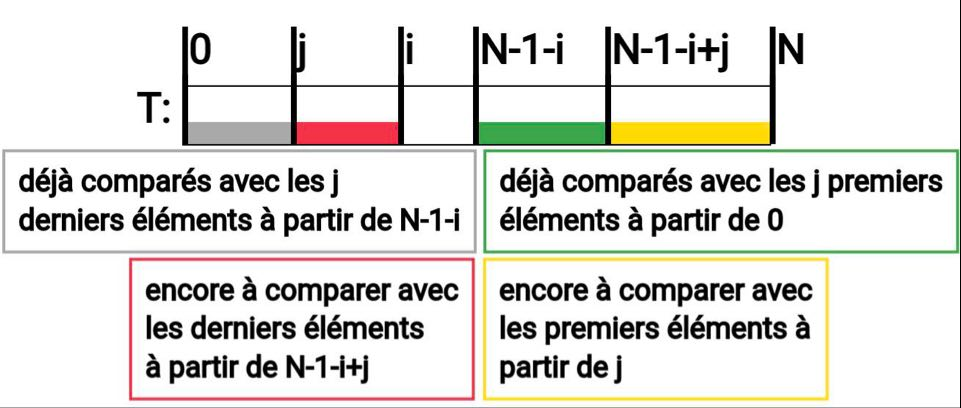
\includegraphics[scale=0.4]{invariant_sp2.jpg}
  \caption{Invariant SP2}
\end{figure}

$$Inv: N=N_0\wedge T=T_0\wedge 0\leq j \leq i\wedge MemeSSTableau(T,N,i)=1$$
\subsection{Gardiens de boucle}
\begin{itemize}
  \item SP1: $i<N-1$
  \item SP2: $j\leq i$
\end{itemize}
\subsection{Critères d'arrêt}
\begin{itemize}
  \item SP1: $i=N-1$
  \item SP2: $j=i+1 \vee T[j]\neq T[N-1-i+j]$
\end{itemize}
\subsection{Fonctions de terminaison}
\begin{itemize}
  \item SP1: $N-1-i$
  \item SP2: $i+1-j$
\end{itemize}

\section{Code}

\subsection{Schéma de la fonction "EgaliteSSTab"}
\begin{lstlisting}[caption={Schéma de la fonction "EgaliteSSTab"}]
  {
    //Initilisation des variables

    //Début SP1

    //SP2

    //Fin SP1

    return taille_sous_tableau;
  }//fin EgaliteSSTab
\end{lstlisting}

\subsubsection{Initialisation des variables}
Cet extrait de code présente le début de notre fonction qui est constitué 
de l'initialisation de nos variables, afin d'arriver au stade où celles-ci vérifient les pré-conditions du SP 1.
\begin{lstlisting}[caption={Initialisation des variables}]
  (>\textcolor[HTML]{17983b}{\{Pré: $T_{init}\wedge N>1\}$}<)
  assert(T!=NULL && N>1);
  unsigned int i=0, j;
  (>\textcolor[HTML]{17983b}{\{$T=T_0\wedge N=N_0\wedge i=0\wedge j_{init}$\}}<)
  int taille_sous_tableau=0, est_pref_et_suf=1;
  (>\textcolor[HTML]{17983b}{\{$T=T_0\wedge N=N_0\wedge i=0\wedge j_{init}\wedge taille\_sous\_tableau=0\wedge est\_pref\_et\_suf=1$\}}<)
\end{lstlisting}
Les pré-conditions du SP1 correspondent bien au conditions de notre prédicat final.

\subsubsection{Sous-problème 1}
\begin{lstlisting}[caption={Sous-problème 1}]
  (>\textcolor[HTML]{17983b}{\{$Inv: T=T_0\wedge N=N_0\wedge 0\leq i\leq N-1$\}}<)
  while(i<N-1){
      (>\textcolor[HTML]{17983b}{\{$Inv\wedge B: T=T_0\wedge N=N_0\wedge 0\leq i\leq N-2$\}}<)
      j=0;
      est_pref_et_suf=1;
      (>\textcolor[HTML]{17983b}{\{$T=T_0\wedge N=N_0\wedge j=0\leq i \leq N-2$\}}<)
      (>\textcolor[HTML]{17983b}{\{Pré SP2: $T=T_0\wedge N=N_0\wedge j=0\wedge est\_pref\_et\_suf=1$\}}<)

      //SP2

      (>\textcolor[HTML]{17983b}{\{Post SP2: $T=T_0\wedge N=N_0\wedge est\_pref\_et\_suf=MemeSSTableau(T, N, i)$\}}<)

      if(est_pref_et_suf==1)
          taille_sous_tableau=i+1;
      (>\textcolor[HTML]{17983b}{\{Post SP1 : $T = T_0 \wedge N = N_0 \wedge est\_pref\_et\_suf = MemeSSTableau(T, N, i)$\}}<)
      i++;
      (>\textcolor[HTML]{17983b}{\{$T=T_0\wedge N=N_0\wedge 0\leq i\leq N-1\wedge est\_pref\_et\_suf = MemeSSTableau(T, N, i)$\}}<)
  }//fin while
\end{lstlisting}

\newpage

\subsubsection{Sous-problème 2}
\begin{lstlisting}[caption={Sous-problème 2}]
  (>\textcolor[HTML]{17983b}{\{Pré SP2: $T=T_0\wedge N=N_0\wedge j=0\wedge est\_pref\_et\_suf=1$\}}<)
  (>\textcolor[HTML]{17983b}{\{$Inv:T=T_0\wedge N=N_0\wedge 0\leq j\leq i+1\wedge MemeSSTableau(T, N, i) = 1$\}}<)
  while(j<=i){
      (>\textcolor[HTML]{17983b}{\{$Inv\wedge B:T=T_0\wedge N=N_0\wedge 0\leq j\leq i\wedge MemeSSTableau(T, N, i) = 1$\}}<)
      if(T[j]!=T[N-i+j-1]){
          est_pref_et_suf=0;
          j=i;
      }
      (>\textcolor[HTML]{17983b}{\{$T=T_0\wedge N=N_0\wedge 0\leq j\leq i+1\wedge est\_pref\_et\_suf=MemeSSTableau(T, N, i)$\}}<)
      j++;
      (>\textcolor[HTML]{17983b}{\{$T=T_0\wedge N=N_0\wedge 0\leq j\leq i\wedge est\_pref\_et\_suf=MemeSSTableau(T, N, i)$\}}<)
  }
  (>\textcolor[HTML]{17983b}{\{Post SP2:$T=T_0\wedge N=N_0\wedge est\_pref\_et\_suf=MemeSSTableau(T, N, i)$\}}<)
\end{lstlisting}


\section{Complexité}
On va découper la complexité en plusieurs segments et ensuite on va les additionner.
La première partie est l'initialisation des variables et vu qu'on en déclare 4 $$T_A(N)=4$$\\
Ensuite, on a la première boucle et par la règle 5, on a $$T_B(N)=\sum_{i=0}^{N-1}(4+T_C(i))$$ Dans ce cas-ci, le "4" représente l'initialisation des variables et le $T_C(i)$ est la deuxième boucle.
Pour la deuxième boucle, on a $$T_C(i)=\sum_{j=0}^i1$$\\
On a donc $$T_C(i)=i$$\\
On revient à la première boucle $$T_B(N)=\sum_{i=0}^{N-1}(4+i)\Leftrightarrow T_B(N)=\frac{N^2+7N}{2}$$\\
Enfin, en additionnant le tout, on obtient $$T(N)=\frac{N^2+7N+8}{2}$$\\
Dans ce cas ci, notre complexité $T(N)$ est majorée par $O(N^2)$. On peut donc en conclure que la fonction est de complexité quadratique.

\end{document}
